% Ryan Logsdon and Adam Jarvis
% March 28, 2023 
% logsdori@mail.uc.edu, jarvisar@mail.uc.edu
% CS 5058/6158 Data Security and Privacy

\documentclass[sigconf]{acmart}

\usepackage{booktabs} % For formal tables

% additional packages by Boyang
\usepackage{graphicx}
\usepackage{array}
\usepackage{amsmath}
\usepackage[ruled, vlined, linesnumbered]{algorithm2e}
\usepackage{algorithmic}
\usepackage{amssymb} %\varnothing
\usepackage{framed,multicol} 
\usepackage{subfigure}

\usepackage[framemethod=TikZ]{mdframed}
%\mdfsetup{frametitlealignment=\center}

%\renewcommand{\algorithmicrequire}{\textbf{Input:}}
%\renewcommand{\algorithmicensure}{\textbf{Output:}}

% Copyright
%\setcopyright{none}
%\setcopyright{acmcopyright}
%\setcopyright{acmlicensed}
\setcopyright{rightsretained}
%\setcopyright{usgov}
%\setcopyright{usgovmixed}
%\setcopyright{cagov}
%\setcopyright{cagovmixed}


% DOI
\acmDOI{10.1145/3317549.3323409}

% ISBN
\acmISBN{978-1-4503-6726-4/19/05}

%Conference
\acmConference[ACM NS'23]{ACM Conference on Network Security}{April 4-6, 2023}{New York, NY, USA} 

\acmYear{2023}
\copyrightyear{2023}



\begin{document}
\title{Evaluation and Analysis of HomeSnitch}
%\titlenote{Produces the permission block, and
%  copyright information}
%\subtitle{This is a Draft}
%\subtitlenote{The full version of the author's guide is available as
%  \texttt{acmart.pdf} document}


\author{Adam Jarvis}
\affiliation{%
  \institution{M12857829}
}

\author{Ryan Logsdon}
\affiliation{%
  \institution{M13336638} 
}

%\author{G.K.M. Tobin}
%\authornote{The secretary disavows any knowledge of this author's actions.}
%\affiliation{%
%  \institution{Institute for Clarity in Documentation}
%  \streetaddress{P.O. Box 1212}
%  \city{Dublin} 
%  \state{Ohio} 
%  \postcode{43017-6221}
%}
%\email{webmaster@marysville-ohio.com}

% The default list of authors is too long for headers}



\begin{abstract}
 The increasing availability and accessibility of smart home IoT devices has made them a staple within modern society. Although these tools seek to provide end users with increased connectivity and convenience, the lack of industry guidelines surrounding network-based security have allowed these devices to become a threat to a users privacy and security. In order to enhance smart home transparency and control, HomeSnitch was created as a building block of smart home device security \cite{Enck}. HomeSnitch seeks to classify IoT communication based upon is semantic behavior (e.g., heartbeat, firmware check, motion detection) through the application-layer dialog between clients and servers. This device is able to identify behaviours using features of connection-oriented application data unit exchanges, while ignoring encrypted payload content. We explore why this system is so important in the area of network security, how the system is built, and explore the results and limitations of HomeSnitch as a readily available solution. 
\end{abstract}

%
% The code below should be generated by the tool at
% http://dl.acm.org/ccs.cfm
% Please copy and paste the code instead of the example below. 
%
\begin{CCSXML}
<ccs2012>
   <concept>
       <concept_id>10003033.10003099.10003102</concept_id>
       <concept_desc>Networks~Programmable networks</concept_desc>
       <concept_significance>500</concept_significance>
       </concept>
   <concept>
       <concept_id>10010147</concept_id>
       <concept_desc>Computing methodologies</concept_desc>
       <concept_significance>500</concept_significance>
       </concept>
   <concept>
       <concept_id>10002978.10003014</concept_id>
       <concept_desc>Security and privacy~Network security</concept_desc>
       <concept_significance>500</concept_significance>
       </concept>
 </ccs2012>
\end{CCSXML}

\ccsdesc[500]{Networks~Programmable networks}
\ccsdesc[500]{Computing methodologies~Bagging}
\ccsdesc[500]{Security and privacy~Network security}


\maketitle

\section{Introduction}
\label{sec:intro}
The integration of the Internet-Of-Things (IoT) devices within the residential environment has become increasingly prevalent over the past two decades. Everyday consumers are aware of the vast amount of automation that can be acquired through devices carrying wireless sensors and monitors. Many of these devices seek to provide increased home security through cameras, audio collection,  and alarms. Moreover, the connection of these various devices creates an ever-growing web of wireless communication. However, as the pervasiveness of IoT devices was estimated to be 50 billion devices in 2020 \cite{Helen}, risk is being introduced as devices attach to these often-insecure networks. 
    
The issue HomeSnitch attempts to solve is exactly this: a compromised or misbehaving smart home device may attack other network hosts, but it may also eavesdrop on the physical home environment \cite{Enck}. The challenge with this problem is identifying when a devices behavior is acceptable and when it has become malicious. For the majority of devices, it is not necessary to increase security when the device is in use, but rather monitor potential eavesdropping activities when the device is idle. Simple solutions such as turning a device off may seem sufficient, however, a long-term solution to access control is necessary to enhance network security. 

HomeSnitch functions as a building block for improving transparency and control over the network communications between smart home devices. This solution provides an ability to classify and control semantic behaviors using features that represent the application-layer dialogue between clients and servers \cite{Enck}. Many smart home devices have poor authentication mechanisms and software vulnerabilities that present threats due to unexpected behavior implemented by manufacturers. Overcoming the challenge of diagnosing device behavior while respecting encrypted payload data is crucial to providing transparency and control for the end user.  

The remainder of this paper proceeds as follows: Section 2 details the HomeSnitch model and the threat it attempts to solve. Section 3 details the techniques HomeSnitch utilizes to solve this problem. Section 4 provides an evaluation of experimental results. Section 5 offers a discussion of the limitations of the study and potential future research. Section 6 concludes. 
\section{System and Threat Model}
\label{sec:related}
To understand the HomeSnitch solution, it is important to define the threat model and assumptions it was designed to overcome. This device is designed for a residential home network setup consisting of sensors, actuators, and smart objects, both wired and wirelessly connected to a consumer-grade router.  Assumptions about this network include that devices contain default credentials, lack sufficient security protocols, enable over-privilege and contain un-patched vulnerabilities. The threat can compromise smart home devices either by directly connecting to them through Nat hole punching \cite{Vijay}, lateral pivoting from other compromised devices, gaining physical control of the device \cite{Nitesh}, or abusing cloud-based control. 

The goal of a malicious threat is to exploit devices to cause physical effects, such as turning off an alarm. Subsequently, an adversary may steal data, enable remote surveillance, steal credentials, or compromise other network devices. The attackers may launch an attack, or abuse server-side privileges on the specific service-provider for a device. The authors believe that defending attacks without the cooperation of the device is a sufficiently hard problem since traditional security approaches involve scanning for vulnerabilities, enabling fine-grained permissions on the host, and patching vulnerabilities. A smart home network of devices cannot employ any of these approaches as defense \cite{Enck}. HomeSnitch uses IP connection-oriented protocols to prevent such attacks. 

\section{Current Solution}
\begin{figure}[h]
\centering
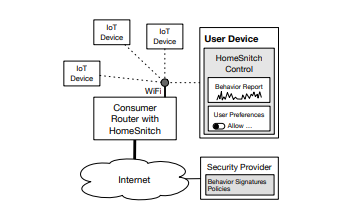
\includegraphics[width=0.5\textwidth]{Figure 1.PNG}
\caption{HomeSnitch provides a building block for transparency and control of IoT device behaviors \cite{Enck}}
\label{fig:example}
\end{figure}


This section describes how HomeSnitch, as depicted in Figures 1 and 2, seeks to solve the issue of increasing transparency and control through the use of semantic behaviors. HomeSnitch defines behaviors through application data unit (ADU) exchanges which describe an application behavior as a semantic triple the classifies the vendor and model of a device as well as the activity it is performing. The system uses adudump \cite{Jeff} for continuous measurement of application-level data from network flows. Since adudump only utilizes TCP/IP packet header traces to construct a model of the dialog between a server and the client, encryption at the application layer was no longer a barrier. Therefore, application data units were sufficient to accurately distinguish between behaviors. 

In order to classify ADUs by feature, the authors utilized supervised machine learning to classify network flows. Due to the limited complexity of IoT devices, traffic is predominately sequential with the server and clients taking turns. This allows HomeSnitch to gather statistics from each sequential turn, such as total data sent and received, data sent per sequence, and total time of connection. Overall, it was determined that average bytes, max bytes, and aggregate bytes from IoT devices were the dominant feature used within the supervised learning algorithm. 

The authors chose to utilize the Random Forest algorithm for classification because it leverages both ensemble and averaging methods to build several estimators independently and then average their predictions \cite{Fabian}. Moreover, by using this approach, there is an increased resistance to under-fitting. To supply training data-sets for the algorithm, DBSCAN, a clustering based density sampling algorithm, was utilized \cite{Martin, Fabian}.

A major barrier to the development of HomeSnitch was the ability to detect new behaviors for new devices after the initial implementation. To overcome this, a security service provider was used to share features and expand the set of supported behaviors. However, a provider that sends information out of the home network raise concerns of privacy and data quality. To ensure privacy, HomeSnitch limits data collection to the features and labels collected within a smart home IoT deployment \cite{Enck}. 

\begin{figure}[h]
\centering
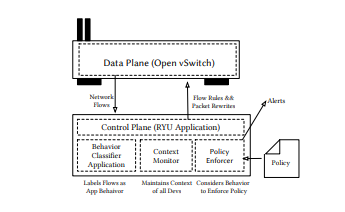
\includegraphics[width=0.5\textwidth]{Figure 2.PNG}
\caption{HomeSnitch leverages a fine-grained behavior
classification approach to provide context for effective policy enforcement and access control. \cite{Enck}}
\label{fig:example}
\end{figure}

Based upon the classification of behaviors from the machine learning algorithm, HomeSnitch is able to enact policies to provide access control to the network traffic. For example, a device behavior that has been classified as normal, such as a Ring Doorbell uploading a small motion detection, will be permitted by the policy. This action would be classified in an ADU semantic triplet as "drop Ring-Doorbell, [Ring,Doorbell,Motion-Upload] (T: 0100-0300)". However, an unusual action will be denied, such as a smart lock being opened when the management device is not on the network, which would be classified as "reject LockState-Lock, [Lockstate,Lock,Unlock], (M: notpresent)". The entirety of the context free grammar for the HomeSnitch policy language is provided within Appendix A of the paper \cite{Enck}.

HomeSnitch was built upon a wireless access point running an open source firmware that supports a virtual switch and the OpenFlow SDN protocol. The implementation relies primarily on a data plane and control plane. The data plane uses a Linksys router that is configured to use simultaneous dual band with support for 2.4 GHz and 5 GHz. An Open vSwitch Support bridge was used to bind WiFi and local Ethernet interfaces allowing OpenFlow to manage wireless connected devices. The control plane  was implemented using the custom Software Defined Networking (SDN) Security Orchestrator on a Raspberry Pi 3 Model B single board computer connected via Ethernet. Using an Ubuntu 16.04 Operating System, a Ryu management application was derived to enact the access control derived from the classification policies described above. 

Future directions for the HomeSnitch system could involve expanding the number of supported devices and behaviors, as well as improving the accuracy of the machine learning algorithm. Additionally, incorporating natural language processing (NLP) techniques could enhance the ability of the system to understand and interpret user intent and input. The authors suggest that HomeSnitch could also be extended to provide users with greater visibility and control over their data, as well as offering more sophisticated policy-based access control mechanisms \cite{Enck}. Furthermore, future research could explore the application of HomeSnitch to other domains beyond the smart home, such as in industrial control systems or healthcare environments. Ultimately, ongoing developments in the IoT space will require continued innovation and refinement of security and privacy solutions such as HomeSnitch to keep pace with evolving threats and use cases.

\section{Evaluation and Experimental Results}

To evaluate the feasibility of HomeSnitch as a means of providing access control and transparency, the authors tested the solution within a residential IoT network. The performance was evaluated against its accuracy in identifying and classifying smart home IoT device behaviors, its performance impact on throughput, and the amount of training needed for the machine algorithm to classify different behaviors. The experiment was conducted on a network consisting of 46 devices registering 148 semantic behaviors on over 2,000 connections to cloud endpoints. 

To evaluate accuracy, the Random Forest algorithm for classification was compared against kNN (used in Peek-A-Boo \cite{Abbas}) and Gradient Boost (used in \cite{six}) for the same data set. Results from these tests revealed that Random Forest received higher ratings for accuracy, recall and total F1 Score, at 99.69\%, 94.66\% and 92.92\% respectively.

To evaluate performance, a physical and emulated test bed were utilized to simulate the network flow of many IoT devices. An iPerf Toolkit was used to actively measure throughput and jitter during the experiment. Due to the SDN controller implementation, a total of 100ms latency overhead was observed for HomeSnitch, however this resulted in minimal impact for throughput, which retained 97.01\% of its performance. 

To evaluate the amount of training required by the solution, a test-training set approach iterated through 200 samples of behavior classes. During each iteration, samples were incrementally introduced into the system and the classification accuracy was measured. Next, a prediction score was calculated for the remaining unlabeled samples from the behavior class. Through this method, it was determined that an average of 58 to 63 samples were necessary to achieve 90\% and 95\% prediction confidence. 

HomeSnitch provides a web interface to apply policy actions for specific IoT devices at the discretion of the end-user. Testing of this feature included enabling the motion detection of a Ring Doorbell. When the motion detection was triggered, an alert of malicious behavior was not given to the user or logged in the application. Moreover, the 407 packets observed were able to flow unrestricted to the Ring servers. Another rule was implemented to restrict a D-Link Motion sensor from uploading motion sensing data. As a result, after being triggered 26 packets were dropped. However, after the rule expired, the motion sensor uploaded the buffered motion data. This demonstrates that the policies enacted through the behavior classification model must be aware of the buffering and communication model of each IoT device. 

Overall, the HomeSnitch solution was able to derive a system capable of semantically categorizing IoT device behavior in a residential environment. Through testing against malicious behavior, the system was able to offer insight to a user that a device was compromised via a malicious attack. Moreover, the context free grammar utilized for policy creation was able to effectively regulate access control across numerous devices. With further analysis, it was determined that the few inconsistencies witnessed during the experiment were during heartbeat activities of IoT devices. These activities account for a vast majority of device activity, while also presenting the smallest threat to attack. Therefore, the HomeSnitch solution appears to provide a thorough defense mechanism against the network security pitfalls present within smart-home devices. 

\section{Limitations}

One of the major limitations of the HomeSnitch solution is its susceptibility to Mimicry Attacks. Supervised machine learning leverages classifiers to identify traffic patterns that represent device behaviors, and an informed adversary that is able to compromise a device and mimic the traffic patterns of permitted behaviors would be able to bypass the classification system. However, in order to successfully overcome the policy rules, an attacker must learn the contents of the content grammar. The authors propose complementary approaches including device identity, anti-tampering and device attestation as potential solutions to this limitation. 

Another limitation of this device is the requirement of capturing the full network flow for precise classification. To enable real-time enforcement, historical flow data must be considered to modify instructions. Given the simplistic communication methods of these IoT devices, a modified approach would be feasible to predict real-time behaviors without increasing latency. The authors propose the construction of a stochastic model as a topic for future research around this limitation.

While the HomeSnitch solution offers a promising approach to securing IoT devices, the use of machine learning also introduces a potential risk of false positives and/or false negatives. False positives occur when the system incorrectly identifies benign traffic as malicious, while false negatives occur when the system fails to detect actual malicious traffic. This can have serious consequences, as false positives can lead to unnecessary security measures that disrupt legitimate device activity, while false negatives can leave the network vulnerable to attacks. Because of this, it is important to carefully evaluate the performance of machine learning models and implement additional functionality to mitigate the risk of false positives and false negatives.

Finally, in order to create ease-of-use for the end-user, HomeSnitch needs to become integrated within the router and provide capabilities for users to allow and disallow activities of specific IoT devices. Future work is needed to establish the feasibility of institutional guidelines being implemented to increase network security of currently unregulated devices. 
\section{Conclusion} 
\label{sec:conclusion}

HomeSnitch presents a feasible building block for enhanced transparency and access control for end-users by classifying smart home device communication by their semantic behaviors. Software-defined networking is used to monitor client-server communication and classify device behaviors. This approach enables HomeSnitch to ensure the security of encrypted data and proprietary protocols being utilized throughout smart home devices. Overall, HomeSnitch proved to provide an accurate means of labeling device behavior and defining policies to alert users of potential malicious attacks.

\bibliographystyle{ACM-Reference-Format}
\bibliography{main} 
%\bibliography{sample-bibliography} 

\newpage

%\input{appendix}

\end{document}
